\documentclass{article}

\title{Praca magisterska, wersja robocza}
\date{2015-09-02}
\author{Hubert Guzera}



\usepackage{polski}
\usepackage[utf8]{inputenc}
\usepackage{amsthm}
\usepackage[intlimits]{amsmath}
\usepackage{natbib}
\usepackage{graphicx}
\usepackage{tikz}


\usetikzlibrary{shapes.callouts}
\tikzset{
  level/.style   = { ultra thick, blue },
  connect/.style = { dashed, gray },
  connect_k/.style = { dashed, red },
  notice/.style  = { draw, rectangle callout, callout relative pointer={#1} },
  label/.style   = { text width=2cm }
}

\usetikzlibrary{calc,trees,positioning,arrows,chains,shapes.geometric,%
    decorations.pathreplacing,decorations.pathmorphing,shapes,%
    matrix,shapes.symbols}

\tikzset{
>=stealth',
  punktchain/.style={
    rectangle, 
    rounded corners, 
    % fill=black!10,
    draw=black, very thick,
    text width=10em, 
    minimum height=3em, 
    text centered, 
    on chain},
  line/.style={draw, thick, <-},
  element/.style={
    tape,
    top color=white,
    bottom color=blue!50!black!60!,
    minimum width=8em,
    draw=blue!40!black!90, very thick,
    text width=10em, 
    minimum height=3.5em, 
    text centered, 
    on chain},
  every join/.style={->, thick,shorten >=1pt},
  decoration={brace},
  tuborg/.style={decorate},
  tubnode/.style={midway, right=2pt},
}

\begin{document}



\maketitle


\pagenumbering{gobble}

\pagenumbering{arabic}

\paragraph{Wprowadzenie} \mbox{}\\

Wal-Mart, amerykański gigant handlowy, co godzinę umieszcza w swoich bazach danych 2.5 petabajtów danych, pochodzących z blisko miliona transakcji. I nie jest wyjątkiem - przeciętna ilość danych przechowywanych przez przedsiębiorstwa w Stanach Zjednoczonych jest większa niż zbiory Biblioteki Kongresu (szacowane na 235 terabajtów). W erze informacji większość z danych generowanych przez konsumentów trafia na serwery tej bądź innej firmy, w formie historii transakcji, koordynatu GPS czy zdjęcia. 

Często informacje te zbierane są przypadkiem - ze względu na prowadzenie rachunkowości, specyfikę świadczonych usług, lub też względy archiwizacyjne. Jednak wydobycie z nich \textit{wiedzy} może stanowić źródło znaczącej przewagi konkurencyjnej.  Jak wskazują Brynjolfsson, Hitt i Kim \cite{Brynjolfsson2011}, przedsiębiorstwa podejmujące decyzje na podstawie analizy dużych zbiorów danych (\textit{data driven decision making}) osiągają efektywność o 5-6 proc. większą niż grupa porównawcza. Mają także większy zwrot z kapitału i wycenę rynkową - jednym słowem, radzą sobie lepiej. Nic więc dziwnego, że coraz częściej data analytics staje się priorytetem wśród dużych spółek. Skalę popularności business intelligence unaocznia badanie PwC \cite{PwC2014}, według którego 44 proc. CEO planuje oparcie rozwoju firmy o inwestycje w tej dziedzinie. 

Ale dzisiejsze zastosowania \textit{big data} to tylko preludium do tego, co czeka nas w przyszłości. Trwający równolegle trend robotyzacyjny spowoduje, że w ciągu 20 lat w przedsiębiorstwie zamiast kierowców możemy zarządzać flotą autonomicznych pojazdów, a magazynierów zastąpią roboty. Fakt, że Google i Daimler już testują takie auta nie pozwala na nazwanie tego science-fiction. Według Carla Freya i Michela Osborne'a z Uniwersytetu w Oxfordzie \cite{Frey2013}, blisko 47 proc. miejsc pracy jest zagrożonych komputeryzacją. Większość z nich to zawody wykonujące rutynowe, mechaniczne czynności, ale postęp technologiczny powoduje, że na tej liście znajdują się też prace wymagające umiejętności kognitywnych i wnioskowania - jak pracownicy biurowi, analitycy czy operatorzy. 

Jeśli więc w jednej strony mamy do czynienia z flotą autonomicznych pojazdów, z a drugiej z petabajtami informacji o tym gdzie i co kupują nasi klienci, możemy znaleźć się w sytuacji, gdzie koordynacja łańcucha dostaw będzie wykraczać poza możliwości człowieka. Dla komputera, wyprognozowanie popytu na podstawie danych i zaplanowanie dostaw nie będzie żadnym problemem. Potwierdza to The McKinsey Global Institute \cite{McKinsey&Company2011}, który wskazuje, że coraz częściej maszyny będą zastępować ludzi w podejmowaniu decyzji i brać udział w sterowaniu przedsiębiorstwem. 

W teorii, ze względu na możliwość przeprowadzania złożonych obliczeń i analizy gigabajtów danych, decyzje te będą trafniejsze i poprawią efektywność przedsiębiorstwa. 

Niniejsza praca ma na celu skonfrontowanie tej hipotezy. Po pierwsze, poprzez zaproponowanie jednego z wielu możliwych algorytmów optymalizacji działania przedsiębiorstwa poprzez wykorzystanie istniejących technik \textit{modelowania predykcyjnego}. Po drugie przez sprawdzenie, jak tak podejmowane decyzje będą wpływać na funkcjonowanie przedsiębiorstwa i czy będzie ono funkcjonować efektywniej, niż gdyby zastosować w nim dotychczasowe praktyki biznesowe.

\newpage
 
\tableofcontents

\newpage


\section{Cel, założenia i podstawy teoretyczne pracy}
\subsection{Koncepcja pracy}

Praca ma na celu zaproponowanie algorytmu optymalizacji podejmowania decyzji w przedsiębiorstwie na podstawie modelowania predyktywnego oraz sprawdzenie, jak zaimplementowanie takiego algorytmu wpływa na efektywność firmy.  

Przyjmując, że optymalizowane przedsiębiorstwo z sektora FMCG zajmuje zarówno produkcją, jak i dystrybucją towarów do sklepów detalicznych, będziemy starali się w prognozować w krótkiej perspektywie wolumen sprzedaży w każdym ze sklepów. Wykorzystaną wiedzę wykorzystamy do optymalizacji procesów logistycznych, tj. zbudowanie takich tras dostaw i alokację wśród nich wolumenów produktów, żeby zysk firmy był jak największy. 

W celu zaprezentowania wyniku działania powstałego w ten sposób algorytmu, zostanie zbudowany model wieloagentowy symulujący rynek i zachowania klientów. Z jego pomocą sprawdzimy funkcjonowanie algorytmu w trzech przypadkach załozeń: 

\begin{enumerate} 
	\item Cena produktu jest stała, a w łańcuchu produkcyjnym nie występują efekty skali 
	\item Cena produktu jest stała, a w łańcuchu produkcyjnym występują efekty skali
	\item Cena produktu jest decyzją przedsiębiorstwa, a w łańcuchu produkcyjnym występują efekty skali
\end{enumerate}


\subsection{Podstawy teoretyczne}
\paragraph{Przedsiębiorstwo jako system wieloagentowy} \mbox{}\\
Na możliwość wykorzystania modeli wieloagentowych do badania i zarządzania systemami logistycznymi wskazują m.in. Moyaux et al, 2006 \cite{Moyaux2006}  czy Kawa, 2010 \cite{Kawa2010}. W swoich pracach zauważyli oni, że  \textit{producenci},  \textit{dostawcy} i  \textit{odbiorcy} i inni uczestnicy łańcucha logistycznego mogą być opisani jako sieć autonomicznych, współpracujących ze sobą agentów. Takie podejście, i wynikająca z niego możliwość wykorzystania modeli wieloagentowych pomaga w rozwiązaniu problemów operacyjnych, na jakie wskazuje Moyaux \cite{Moyaux2006}. Należy bowiem zwrócić uwagę, że w zakresie wyboru tras i zarządzania flotą wieloetapowe łańcuchy dostaw wielu produktów są problemami NP-trudnymi, szczególnie, że decyzje podejmowane lokalnie są współzależne.\footnote{W praktyce, decyzje podjęte na wczesnym etapie łańcucha rezonują na dalsze etapy, co Moyaux opisuje jako "bullwhip effect"} Ponadto, jak zauważa Kawa, w sieci przedsiębiorstw pomiędzy dostawcami kolejnych rzędów (tj. fabryki, magazyny, sklepy) może istnieć wiele połączeń które są wobec siebie konkurencyjne, ponieważ jeden magazyn może zaopatrywać się w wielu fabrykach. Zastosowanie w tej dziedzinie modeli wieloagentowych pozwala więc na zbadanie, jak decyzje podejmowane na jednym z etapów łańcucha dostaw wpłyną na cały system i innych uczestników.  

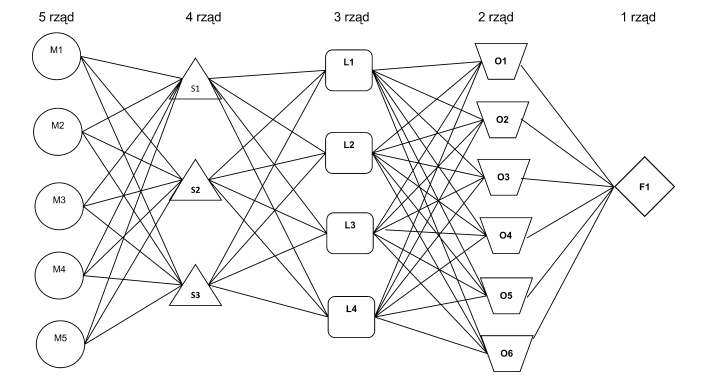
\includegraphics[width=\linewidth]{pictures/siec.png}

W niniejszej pracy stosowane jest rozszerzenie tego podejścia, poprzez zaprogramowanie jako agentów jednostek organizacyjnych przedsiębiorstwa \textit{(fabryka, magazyn, sklep, zarząd)}, które razem tworzą system \textit{(przedsiębiorstwo)}. 

To podejście opiera się na obserwacji, że relacje pomiędzy jednostkami w przedsiębiorstwie są analogiczne do relacji uczestników łańcucha dostaw. Michael Porter zauważył, że działalność przedsiębiorstwa to de facto sekwencja działań, która na każdym ogniwie zwiększa wartość dla odbiorcy. W przypadku firmy mamy więc również do czynienia z opisanym przez Portera łańcuchem wartości (\textit{value chain}).  Ponieważ przedsiębiorstwa często dysponują wieloma duplikującymi swoje działania jednostkami \footnote{Dobrym przykładem są tutaj zakłady samochodowe, które mogą produkować dany model w różnych krajach. Zmiana fabryki powoduje przy tym radykalną zmianę łańcucha dostaw}, łańcuch ten jest nieliniowy i w jego przypadku mamy do czynienia z podobnymi wyzwaniami co w łańcuchu logistycznym.

Zdefiniowanie jako agentów poszczególnych jednostkek przedsiębiorstwa jest przy tym spójne z określoną przez Wooldridge i Jennings charakterystyką agenta, który według ich postulatów posiada : 
	\begin{itemize}
		\item autonomię - poszczególne jednostki przedsiębiorstwa podążają za strategią i celami narzuconymi przez zarząd, ale mają zazwyczaj swobodę w podejmowaniu decyzji mających na celu ich realizację
		\item zdolności do komunikacji - jednostki przedsiębiorstwa komunikują się z otoczeniem (relacje z klientami) oraz między sobą (raportowanie do zarządu, spotkania), a w ramach pomiędzy jednostkami przedsiębiorstwa istnieje asymetria informacji
		\item reaktywność - jednostki przedsiębiorstwa reagują na zmiany rynkowe oraz zmiany wewnętrz przedsiębiorstwa
	 	\item proaktywność - jednostki przedsiębiorstwa podejmują inicjatywy mające na celu zwiększyć wartość przedsiębiorstwa, jak działalność innowacyjna bądź ekspansja. 
	\end{itemize}
 
 Dlatego w niniejszej pracy będziemy rozważać model wieloagentowy, w którym według założeń na przedsiebiorstwo składać się będzie szereg autonomicznych agentów,
	\begin{itemize} 
		\item \textit{fabryk} $\in$ $FA = \{fa_1,fa_2,fa_3..fa_m\} $ 
		\item \textit{magazynów} $\in$ $MA = \{ma_1,ma_2,ma_3..ma_k\} $ 
		\item \textit{sklepów} $\in$ $SK = \{sk_1,sk_2,sk_3..sk_i\} $
		\item \textit{zarząd}, pełniący rolę centralnego koordynatora i przechowujący wszystkie powyższe $\in$ $ZA = \{FA,MA,SK\} $
	\end{itemize}

przez które kolejno będzie musiał przejść produkt zanim będzie mógł być zakupiony przez klienta. Rozpatrując ten system w proponowanym przez Kawa, 2013 kontekście teorii grafów oznacza to, że łańcuch produkcyjny może składać się z $m= $ $n\choose 1 $ $ \times $ $k\choose 1 $ $ \times $ $i\choose 1 $ kombinacji $d_m$ połączeń pomiędzy jednostkami przedsiębiorstwa. Jak zauważa Kawa, każde z tych połączeń będzie miało swoją maksymalną przepustowość oraz koszt $k_d \in f[d]$, będący sumą kosztów ponoszonych na każdym z ogniw łańcucha wartości. Na krańcach grafu może dojść do sprzedaży towaru i przychodu dla całego systemu - jednak zaopatrzenie sklepu w zbyt dużą ilość towaru doprowadzi do jego zmarnowania i strat. 

\paragraph{Zadanie optymalizacyjne} \mbox{}\\
Dlatego optymalizując działanie przedsiębiorstwa będziemy dążyć do tego, żeby dla danego poziomu produkcji $x$ i zbioru \textit{produktów} $\in$ $PR = \{pr_1,pr_2,pr_3..pr_x\} $ ze zbioru możliwych sterowań (możliwych tras) $<d_1,d_2,d_3..d_m>$ dla każdego z produktów wybrać trasy maksymalizujący wyrażenie

\begin{equation} \label{eq:teoria1}
\max \sum\limits_{pr=1}^x  zysk (cena,d) = \begin{cases}
cena - k_d &\text{jeśli dokonano sprzedaży}\\
k_d &\text{jeśli nie dokonano sprzedaży}
\end{cases}
\end{equation}

\begin{equation*}
 \text{gdzie $k_d \in f[d] \wedge k_d < cena $ }
\end{equation*}

To zadanie optymalizacyjne byłoby trywialne, gdybyśmy mieli doskonałą informację na temat poziomu sprzedaży w każdym ze sklepów w $ t + 1 $. Na taką wiedzę nie możemy liczyć ani w tej pracy, ani w w rzeczywistości, dlatego rozwiązaniem proponowanym w niniejszej pracy jest zastosowanie modelowania predykcyjnego (predictive analytics), w celu prognozowania ilości klientów i ich wyborów w każdym ze sklepów w najbliższych okresach czasu. \footnote{Obecnie w przedsiębiorstwach rzadko stosuje się zaawansowane sposoby prognozowania sprzedaży (\textit{Predictive analytics}), a zarządzanie dostawami odbywa się raczej metodą manualnego uzupełniania zapasów.} 

Ponadto, jak warto zauważyć, nie możemy liczyć na to, że $k_d$ będzie liniowe. Wspominana przez Kawę maksymalna przepustowość każdego z łańcuchów, która w przedsiębiorstwie będzie spowodowana ograniczonymi mocami produkcyjnymi, może spowodować, że funkcja kosztu będzie wykładnicza. W niektórych przypadkach mogą istnieć także korzyści skali, które spowodują, że funkcja będzie logarytmiczna, a całkiem realne jest istnienie obu tych efektów  \footnote{Korzyści skali odczuwalne do pewnego optymalnego poziomu produkcji, powyżej którego brak mocy produkcyjnych powoduje drastyczne powiększanie się kosztów krańcowych}, przez co musimy zakładać, że $f(d)$ może być dowolną funkcją nieliniową.

Trzecim aspektem który trzeba wziąć pod uwagę jest złożoność obliczeniowa. Nawet dla prostego układu, lecz wolumenu produkcji ponad 1000 sztuk sprawdzenie zysku w przypadku wszystkich kombinacji alokacji wymaga olbrzymiej ilości iteracji. Mimo znaczącego wzrostu mocy komputerów w ostatnich latach, wolumeny produkcji w dużych przedsiębiorstwach oraz złożoność tras logistycznych sprawia, że to podejście jest kompletnie niepraktyczne. 

 Proponowany algorytm będzie brał wszystkie te aspekty pod uwagę, a pierwszy z wymienionych problemów rozwiążemy wykorzystując  \textit{modelowanie predykcyjne}.

\paragraph{Modelowanie predykcyjne} \mbox{}\\
Jak wskazuje James, 2013, \textit{modelowanie predykcyjne}\ zakładając, że dysponujemy zbiorem $n$ obserwacji $p$ zmiennych, możemy zbadać ich relację ze zmienną wyjaśnianą $y$ i otrzymać \textit{model}, który dla nowych - nieanalizowanych wcześniej - obserwacji $x_1,x_2..x_n$  zwraca przewidywaną wartość zmiennej objaśnianej \^{y}. Różnorodne metody dzięki którym możemy otrzymać \^{y} James nazywa \textit{Statistical learning} i może być wykorzystany do modelowania predykcyjnego, tj. przewidywania przyszłych wartości \^{y}. 

Zastosowanie metod \textit{statistical learning} w przedsiębiorstwach potwierdza Buckinx, 2007, który wskazywał na możliwość prognozowania lojalności klienta na podstawie wewnętrznych danych o transakcjach, oraz Davenport, który w Harvard Business Review 12/2011 opisuje szereg  \textit{case studies} firm, w których wykorzystuje się istniejące dane o transakcjach do przewidywania przyszłych zakupów klientów. Jednym z podanych przez niego przykładów jest Tesco, które na podstawie zebranych danych przewiduje, jak będzie wyglądał koszyk zakupów klienta podczas następnych zakupów, i odpowiednio wcześnie wysyła mu bony zniżkowe. 

To daje nam podstawy, żeby w przypadku optymalizowanego przedsiębiorstwa zakładać, że dane o każdej transakcji są zapisywane i poza podstawowymi informacjami (produkt, cena, data) zawierają one także dane o kliencie, a cały zbiór danych może być wykorzystany do przewidywania sprzedaży w $t + 1$. Dla każdej transakcji w sklepie dysponujemy więc zbiorem informacji $ X = n \times x_i = <tr_1..tr_k, pr_1.. pr_k,kl_1..kl_k>$ gdzie $tr$ to identyfikatory transakcji (miejsce, data, rodzaj płatności), $pr$ to identyfikatory produktu (nazwa, cena, ilość) oraz $kl$ to identyfikatory klienta (płeć, wiek, zarobki, wykształcenie etc.). 

Na podstawie takiego zbioru danych chcemy przewidzieć popyt na produkty w każdym ze sklepów, co w praktyce oznacza konieczność stworzenia modelu estymującego - 

	\begin{itemize} 
		\item liczbę poszczególnych grup klientów \footnote{Przez "poszczególne grupy klientów" rozumiemy klientów o wspólnej charakterystyce, czyli takich samych zestawach zmiennych identyfikujących $<kl_1..kl_n>$} odwiedzających sklep w $t+1$, gdzie \^{y} $\in R$ 
	\end{itemize}
	oraz w zależności od zastosowanego podejścia
	\begin{itemize} 
		\item prawdopodobieństwo $p$ z jakim klient o danej charakterystyce kupi produkt $pr$, gdzie \^{y} $\in (0,1)$  
		\item jaki produkt wybierze klient o danej charakterystyce, gdzie \^{y} $\in \{pr_1,pr_2..pr_n\}$, a $pr_i$ to dostępny produkt.
	\end{itemize}

Jak wskazuje James, zmienna objaśniana \^{y} może przyjąć formę liczby rzeczywistej, zmiennej binarnej (1/0), prawdopodobieństwa, \textit{log odds} lub klasy, jednak ze względu na różne dziedziny \^{y}, każdy z tych przypadków różni się metodami które możemy zastosować. Według sugestii James i Hastie, zastosujemy następujące metody

	\begin{itemize} 
		\item do liczby klientów - regresję metodą OLS (\textit{ordinary least squares, metoda najmniejszych kwadratów})
		\item do prawdopodobieństwa zakupu - regresję logistyczną (\textit{logistic regression})
		\item do wyboru produktu- metody klasyfikacyjne - $k-means$ oraz $drzewa klasyfikacyjne$
	\end{itemize}

\newpage

\paragraph{Proponowany algorytm optymalizacyjny} \mbox{}\\
Znając przewidywaną sprzedaż na krańcach grafu, proponowany w niniejszej pracy algorytm rozwiązania powyższego problemu opiera się na obserwacji, że równanie \ref{eq:teoria1} będzie równoważne zapisowi sumującemu po możliwych kombinacjach łańcucha (zamiast dla każdego produktu z osobna).

\begin{equation}  \label{eq:teoria2}
\max \sum\limits_{d=1}^m  zysk(cena) = 
cena \times pr_d -  \ k_d \times pr_d \qquad 
\end{equation}

\begin{equation*}
  \text{ gdzie $pr_d$ to ilość produktów przechodzącym w danym łańcuchu}
\end{equation*}

Ponieważ scieżka $d_m$ składa się z $<fa_m,ma_m,sk_m>$, a koszt ponoszony na całej trasie będzie równie sumie kosztów ponoszonym na każdym z ogniw łańcucha, równanie \ref{eq:teoria2} możemy zapisać jako

\begin{equation} \label{eq:teoria3}
\max \sum\limits_{d=1}^m  zysk(cena) = 
cena \times pr_d -  ( \sum\limits_{j=1} k_j) \times pr_d \qquad 
\end{equation}


gdzie $ k_j$ to koszty ponoszone na każdym z elementów łańcucha wartości (koszty produkcji, magazynowania, transportu, etc.). Te co do zasady są nam znane, więc zostaje nam znalezienie takich wartości $pr_d$ i \textit{ceny} (jeśli nie przyjmujemy założenia danej, stałej ceny) dla których firma będzie osiągać maksymalny zysk. Ze względu na występujące w przedsiębiorstwie współzależności oraz nieliniowość kosztów (korzyści skali) musimy cały układ rozważać łącznie. 

Na przykładzie przedsiębiorstwa = $<fa_1, ma_1, ma_2, sk_1, sk_2, sk_3>$ mamy do czynienia z $m= $ $1\choose 1 $ $ \times $ $2\choose 1 $ $ \times $ $3\choose 1 $ = 6 kombinacji połączeń pomiędzy jednostkami przedsiębiorstwa, przy czym każdy do każdego ze sklepów można przeprowadzić dostawę jedną z dwóch tras. \\ \\ 

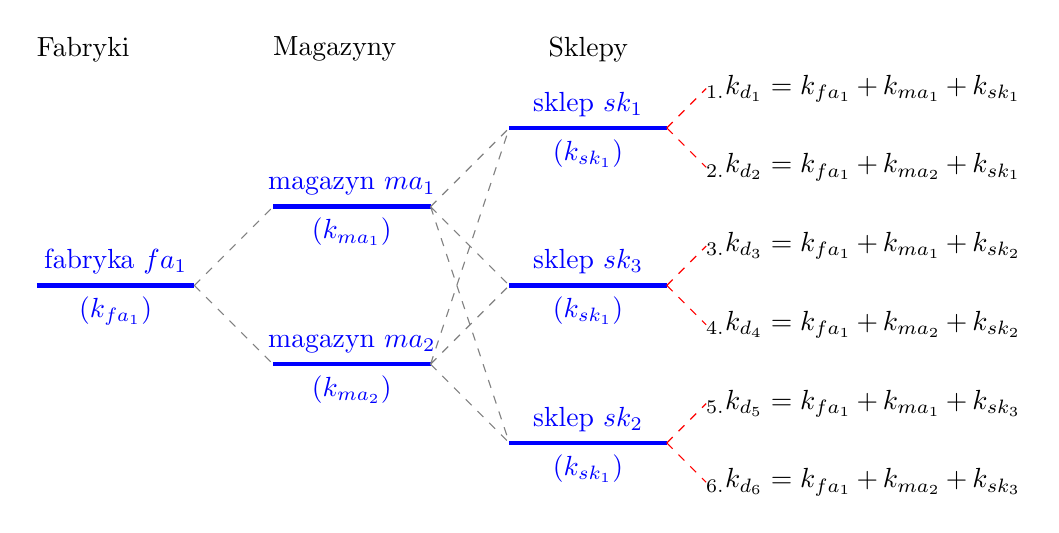
\begin{tikzpicture}
   % Draw all levels

  \draw[level] (0,0) -- node[above] {fabryka  $fa_1$} node[below] {($k_{fa_1}$)}  (2,0);

  \draw[connect] (2,0)  -- (3,-1) (2,0) -- (3,1);
  \draw[level]   (3,1)  -- node[above] {magazyn  $ma_1$} node[below] {($k_{ma_1}$)} (5,1);
  \draw[level]   (3,-1) -- node[above] {magazyn $ma_2$} node[below] {($k_{ma_2}$)} (5,-1);

  \draw[connect] (5,1)    -- (6,2) (5,1) -- (6,0) (5,1) -- (6,-2) (5,1) ;
  \draw[connect] (5,-1)    -- (6,2) (5,-1) -- (6,0) (5,-1) -- (6,-2) (5,-1);

  \draw[level]   (6,2)  -- node[above] {sklep $sk_1$} node[below] {($k_{sk_1}$)}  (8,2); 
  \draw[level]   (6,-2)  -- node[above] {sklep $sk_2$}node[below] {($k_{sk_1}$)}  (8,-2);
  \draw[level]   (6,0)  -- node[above] {sklep $sk_3$}node[below] {($k_{sk_1}$)}  (8,0);

  \draw[connect_k] (8,2)    -- (8.5,2.5) (8,2) -- (8.5,1.5) (8,2);
  \draw[connect_k] (8,0)    -- (8.5,0.5) (8,0) -- (8.5,-0.5) (8,0);
  \draw[connect_k] (8,-2)    -- (8.5,-2.5) (8,-2) -- (8.5,-1.5) (8,-2);

  \node[text width=4cm] at (10.5,2.5) {$ _{1.} k_{d_1} = k_{fa_1} + k_{ma_1}  + k_{sk_1}  $};
  \node[text width=4cm] at (10.5,1.5) {$ _{2.} k_{d_2} = k_{fa_1} + k_{ma_2}  + k_{sk_1}  $};
  \node[text width=4cm] at (10.5,0.5) {$ _{3.} k_{d_3} = k_{fa_1} + k_{ma_1}  + k_{sk_2}  $};
  \node[text width=4cm] at (10.5,-0.5) {$ _{4.} k_{d_4} = k_{fa_1} + k_{ma_2}  + k_{sk_2}  $};
  \node[text width=4cm] at (10.5,-1.5) {$ _{5.} k_{d_5} = k_{fa_1} + k_{ma_1}  + k_{sk_3}  $};
  \node[text width=4cm] at (10.5,-2.5) {$ _{6.} k_{d_6} = k_{fa_1} + k_{ma_2}  + k_{sk_3}  $};

  % Draw labels
  \node[label] at (1,3)  {Fabryki};
  \node[label] at (4,3)  {Magazyny};
  \node[label] at (7.5,3)  {Sklepy};

  % Draw annotations
\end{tikzpicture}

Ponieważ przewidywany wolumen sprzedaży produktu w każdym z krańców grafu jest nam znana  \footnote{Zakładamy, że dzięki \textit{Predictive analytics} na podstawie poprzednich obserwacji mamy dokładne prognozy dotyczące sprzedaży w $t+1$}, żeby umożliwić obliczenie optymalnego obłożenia każdej z tras prowadzącej do krańcu grafu \footnote{Żeby ograniczyć złożoność obliczeniową staramy się unikać pętli, która sprawdza każdą kombinację, zamiast tego szukając bardziej wyrafinowanych sposobów} możemy dla każdej z tras ilość przechodzących nią produktów zapisać jako 

\begin{equation*}
pr_1 = \alpha pr_{sk_1} , \quad pr_2 = \beta pr_{sk_1} \quad ... \quad  pr_{d-1} = \gamma pr_{sk_i} ,\quad  pr_d = \delta  pr_{sk_i}
\end{equation*}



gdzie $pr_{sk_d}$ to ilość produktów, jakie mają trafić do $sk_d$ krańca grafu leżącego na trasie $d$, a $\alpha,\beta...\delta$ to udział tej trasy w przepływie wszystkich towarów do danego krańca grafu. W ten sposób, równanie  \ref{eq:teoria3} możemy zapisać jako 

\begin{equation} \label{eq:teoria4}
\max \sum\limits_{d=1}^m  zysk(cena) = 
cena \times \alpha pr_{sk_d}-  ( \sum\limits_{j=1} k_j) \times \alpha pr_{sk_d} \qquad 
\end{equation}

Co po rozwinięciu pozwoli nam na sprowadzeniu równania \ref{eq:teoria4} do postaci

\begin{multline} \label{eq:teoria5}
zysk(cena) = \alpha(cena \times pr_{sk_1} - ( \sum\limits_{j=1} k_j) \times pr_{sk_1}) + \\
 ... \ + \delta(cena \times pr_{sk_i} - ( \sum\limits_{j=1} k_j) \times pr_{sk_1})
\end{multline}


jeśli przyjmiemy, że  

\begin{multline*}
a = (cena \times pr_{sk_1} - ( \sum\limits_{j=1} k_j) \times pr_{sk_1}) ... \\
.. b=(cena \times pr_{sk_i} - ( \sum\limits_{j=1} k_j) \times pr_{sk_1})
\end{multline*}

otrzymamy w ten sposób wieloman, w którym współczynniki $a,b$ są nam znane, a pary współczynników $\alpha, \beta$ jednego krańca grafu muszą być mniejsze lub równe 1. \footnote{Warunkiem nie jest "równe 1", ponieważ może istnieć taki udział $\alpha$ w przedziale $<0,1>$ powyżej którego przez nieliniowość funkcji kosztów dostawa może być nieopłacalna}. 

Możemy więc skorzystać  więc z twierdzenia o ekstremach lokalnych funkcji wielu zmiennych z Sydsaeter, 2005, który stwierdza, że jeśli istnieją ekstrema globalne  lub lokalne funkcji, to muszą być one położone w punktach stancjonarnych.  Punktami stancjonarnymi są takie wartości zmiennych ${x_1,x_2...x_n}$ dla których wszystkie pochodne pierwszego rzędu są równe 0. 

Dlatego szukamy rozwiązań układu równań

\begin{align*} 
 \frac{\partial zysk}{\partial \alpha} = 0 \\
\frac{\partial zysk}{\partial \beta} = 0 \\
...\\
\frac{\partial zysk}{\partial \delta} = 0 \\
\end{align*} 

których rozwiązania \\

$\begin{cases} \alpha_1=... \\ \beta_1=...  \\ \delta_1=... \end{cases}	$ $\begin{cases} \alpha_2=... \\ \beta_2=...  \\ \delta_2=... \end{cases}	$  $\qquad $.... $\qquad $ $\begin{cases} \alpha_3=... \\ \beta_3=...  \\ \delta_3=... \end{cases}	$   \\

będą określać możliwe punkty, w których $zysk$ będzie przyjmował wartość największą. Ostatnim krokiem algorytmu będzie więc dla każdego zbioru punktów $\{\alpha_1,\beta_1,\delta_1\} \quad ... \quad \{\alpha_n,\beta_n,\delta_n\}$ sprawdzić wartość funkcji $zysk$ w tych punktach i wybrać z nich wartość największą. \footnote{Wprawdzie możliwe jest także matematyczne wyznaczenie, czy w danym punkcie jest maksimum czy minimum i czy jest to maksimum/minimum globalne, jednak kroki które trzeba przy tym wykonań, m.in. obliczanie Hesjanu, dodadzą niepotrzebnej złożoności obliczeniowej w sytuacji, gdy wartość najmniejszą z tego zbioru można sprawdzić szybą pętlą}

\newpage

\section{Model}
\subsection{Koncepcja modelu}


W ramach pracy zbudowany został model wieloagentowy, który symuluje lokalny rynek na wybrany produkt. W modelu agentami są 
\begin{itemize} 
	\item \textbf{klienci} , których definiują unikalne cechy \footnote{Są to między innymi wiek, zarobki, wykształcenie, zainteresowania - zostanie to dokładnie opisane w dalszej części pracy}  wpływającą na podejmowane przez niego decyzje 
	\item \textbf{przedsiębiorstwo}, sprzedające \textit{produkt} na rynku. Przedsiębiorstwo przy tym ma złożoną strukturę, tj. zamiast działać jako indywidualny agent, składa się z współpracujących ze sobą agentów 
		\begin{itemize}
			\item fabryk
			\item magazynów
			\item sklepów 
			\item zarządu, pełniącego funkcje koordynującą 
		\end{itemize}
	\item \textbf{konkurencji}, również sprzedającej na rynku swoje produkty, ale pasywnej w stosunku do symulowanego przedsiębiorstwa. \footnote{Tj. konkurencja nie zmienia decyzji podjętych przed rozpoczęciem gry, i w założeniu ma stanowić jedynie alternatywę dla konsumentów} 
	\item \textbf{produktów}, które z oczywistych względów nie podejmują decyzji, jednak mają swoją charakterystykę wpływającą na decyzje innych agentów (przede wszystkim konsumentów) oraz przemieszczają się w ramach przedsiębiorstwa. 
\end{itemize}


Żeby dobrze odwzorować kluczowy aspekt lokalizacji i drogi w łańcuchach dostaw, symulowany rynek jest osadzony w \textit{wirutalnym mieście}, czyli każdy agent ma swoją lokalizację w macierzy o wymiarach $x \times y$. Lokalizacja wpływa na działania agenta - klient kupi produkt tylko w sklepie w pobliżu, a dostawa z magazynu do sklepu będzie tym droższa, im bardziej oddalone będą od siebie. 

W każdej jednostce czasu $ t $ klienci z prawdopodobieństwem $ p $ będą potrzebować symulowany produkt, więc odwiedzając bliski sklep, wybiorą jeden z produktów oferowanych przez przedsiębiorstwo i konkurencję. Symulacja wyboru opiera się na danych o preferencjach konsumenckich zebranych w ankiecie na próbie 127 badanych. Ponieważ każdy konsument-agent ma swoje unikalne cechy, w symulowanym procesie wyboru metodą drzewa klasyfikacyjnego przyporządkowujemy wybór, jakiego prawdopodobnie dokonał by jego odpowiednik w świecie rzeczywistym. \footnote{Oczywiście, o wiele lepsze byłoby oparcie pracy o prawdziwe historie transakcji, jednak jest to niemożliwe ze względu na dużą poufność tych danych}

Ponieważ konsument wybiera produkt tylko z gamy dostępnych w sklepie, przed rozpoczęciem tury przedsiębiorstwo musi podjąć szereg decyzji o m.in.
	\begin{itemize}
		\item poziomie produkcji
		\item wolumen dostaw do każdego ze sklepów
		\item rozdzieleniu wolumenów pomiędzy części przedsiębiorstwa  \footnote{Tj. ile z całkowitego wolumenu ma wyprodukować fabryka $A$, a ile fabryka $B$}
	 	\item jaką trasą powinny zostać wysłane dostawy
	\end{itemize}

Każda z tych decyzji będzie miała wpływ na przychody \footnote{Przy założeniu stałej ceny, będą to przede wszystkim \textit{utracone koszty} w przypadku wyczerpania się zapasów w sklepie} oraz koszty firmy. Celem pracy jest zbudowanie algorytmu, który na podstawie dotychczasowej historii transakcji pozwoli symulowanemu przedsiębiorstwu przewidzieć potencjalną sprzedać w czasie $ t +1 $ i ze zbioru możliwych sterowań (wyżej wymienionych decyzji) $<u_{t+1}>$ wybierze takie, które będą maksymalizować zysk. 

\subsection{Zastosowane narzędzia}

Model został zbudowany w języku programowania Python 2.7, z wykorzystaniem elementów języka R oraz następujących bibliotek: 

\begin{center}
\begin{tabular}{ c c c }
 Biblioteka & Źródło & Zastosowanie \\ 
 Sympy & www.sympy.org & Wykorzystanie do obliczeń symbolicznych \\  
 rpy2 & rpy.sourceforge.net & Uruchomienie poleceń języka R   \\
 scikit-learn & scikit-learn.org & Budowania drzew klasyfikacyjnych
\end{tabular}
\end{center}

Kod źródłowy programu dostępny jest pod adresem  \textit{github.com/hubertguzera/master-thesis}

\subsection{Struktura programu}

Program podzielony jest na dwie główne części. Pierwsza odpowiada za stworzenie, w drodze losowań, środowiska w ramach którego toczy się symulacja, wraz z agentami i macierzą lokalizacji. \footnote{Model może pominąć ten część i wczytać pregenerowany świat w celu sprawdzenia różnych scenariuszy w statycznym świecie (ceteris paribus).}

 Druga część przez $t_n$ jednostek czasu egzekwuje decyzje podjęte przez przedsiębiorstwo i symuluje zachowania konsumenckie, zwracając na koniec wyniki (przychody i zysk) przedsiębiorstwa w danej jednostce czasu $t$.


\begin{tikzpicture}
  [node distance=.8cm,
  start chain=going below,]
     \node[punktchain, join] (intro) {Generowanie mapy i lokalizacji};
     \node[punktchain, join] (probf)      {Generowanie konsumentow};
     \node[punktchain, join] (investeringer)      {Generowanie symulowanego przedsiebiorstwa i konkurencji};
     \node[punktchain, join] (perfekt) {Alokacja konsumentów i przedsiębiorstw na mapie};
      \node (asym) [punktchain ]  {Podjęcie przez zarząd decyzji dla przedsiębiorstwa};
      \begin{scope}[start branch=venstre,
        every join/.style={->, thick, shorten <=1pt}, ]
        \node[punktchain, on chain=going left, join=by {<-}]
            (risiko) {Modelowanie predykcyjne popytu na towary};
      \end{scope}
      \begin{scope}[start branch=hoejre,]
      \node (finans) [punktchain, on chain=going right] {Symulowanie wyborów konsumenckich};
    \end{scope}
  \node[punktchain, join,] (disk) {Symulowanie zakupów };
  \node[punktchain, join,] (makro) {Investerings};
  \node[punktchain, join] (konk) {Konklusion};
  % Now that we have finished the main figure let us add some "after-drawings"
  %% First, let us connect (finans) with (disk). We want it to have
  %% square corners.
  \draw[|-,-|,->, thick,] (finans.south) |-+(0,-1em)-| (disk.north);
  % Now, let us add some braches. 
  %% No. 1
  \draw[tuborg] let
    \p1=(risiko.west), \p2=(finans.east) in
    ($(\x1,\y1+2.5em)$) -- ($(\x2,\y2+2.5em)$) node[above, midway]  {Symulacja};
  %% No. 2
  \draw[tuborg, decoration={brace}] let \p1=(disk.north), \p2=(makro.south) in
    ($(2, \y1)$) -- ($(2, \y2)$) node[tubnode] {Analyse};
  %% No. 3
  \draw[tuborg, decoration={brace}] let \p1=(intro.north), \p2=(perfekt.south) in
    ($(2, \y1)$) -- ($(2, \y2)$) node[tubnode] {Przygotowanie agentów};
  \end{tikzpicture}

\subsection{Generowanie mapy}

W celu odpowiedniego odwzorowania kluczowego aspektu lokalizacji i dróg w łańcuchach dostaw, a przy tym wzorując się na podejściu !!!, agenci osadzoni są w przestrzeni, reprezentowaną przez macierz klas o wymiarach (x,y). Dodatkowo, lokalizacje będą połączone drogami, wymusząjąc na agentach poruszanie się tylko w obrębie ścieżek. Dzięki temu, w modelu będziemy mogli wiernie odwzorować wpływ odległości i wyboru trasy na efektywność procesów logistycznych, oraz zależność wyników sklepu od zamieszkującej okolicę populacji.

Każdy element macierzy mapa o wymiarach (x,y) jest instacją klasy lokalizacja o następujących właściwościach 


\begin{tabular}{ c c c }
Zmienna & Dziedzina & Opis \\ 
x & integer & Współrzędna x w macierzy$[x,y]$ \\
y & integer & Współrzędna y w macierzy $[x,y]$ \\
typ & string & Opis typu posesji \\
droga & [integer,integer] & Współrzędne drogi dojazdowej - potrzebne do algorytmu wyszukiwania drogi

\end{tabular}

które generowane są według algorytmu

!!!

Każda mapa wygenerowana przez program spełniać będzie następujące założenia

	\begin{itemize}
		\item Drogi krzyżują się i skręcają tylko pod kątem prostym. Poza skrzyżowaniami, drogi nie mają w sąsiedztwie innych dróg
		\item Inne lokalizacje (domy, sklepy etc.) mogą występować tylko w bezpośrednim sąsiedztwie drogi
		\item Drogi stanowią ciągłą linię, dzięki czemu nie ma punktu, do którego nie dałoby się dojechać z dowolnego miejsca startowego
		\item W regione 2 punktów od skraju mapy nie są generowane ani drogi, ani lokalizacje  \footnote{Jest to zabezpieczenie algorytmu, który w odległości 2 pkt od skraju mapy ma 0 proc. szansy na poprowadzenie ścieżki dalej - ponieważ w przypadku iterowania na skrajach mapy niektóre funkcje (jak sprawdzenie sąsiadujących punktów) mogą odnieść się do współrzędnych poza mapą, powodując błąd programu}
	 	\item Gęstość sieci dróg oraz prawdopodobieństwo występowania zakrętów jest predefiniowana przez użytkownika
	\end{itemize}

\paragraph{Algorytm wyszukiwania drogi} \mbox{}\\

Odległości pomiędzy zadanymi piunktami w modelu są wyszukiwane dynamicznie, na podstawie algorytmu wyszukiwania drogi i zliczaniu ilości punktów w zwracanym przez niego łańcuchu. Algorytm oparty jest na metodach wyszukiwania ścieżek w grafach, dzięki założeniu, że każdy droga o współrzędnej (x,y) na mapie jest punktem grafu, który może sąsiadować z punktami o współrzędnych (x-1,y),(x+1,y),(x,y+1),(x,y-1) \footnote{Punkty (x-1,y-1),(x+1,y-1),(x+1,y+1),(x-1,y+1) wykluczamy przez wcześniejsze założenie, że drogi krzyżują się tylko pod katem prostym}, o ile również są drogrami. Informacje o punktach i sąsiadujących przechowywane są w zmiennej nodes, która jesst słownikiem, dla każdego klucza - punktu na mapie - przechowuje informacje o sąsiadujących punktach, np. (3,2) = [(3,3)(4,3). \footnote{Pewnym ograniczeniem jest, że jako punkty grafu definiujemy tylko drogi, tak więc szukając trasy z punktu A do punktu B de facto szukamy trasy z drogi przy punkcie A do drogi przy punkcie B.}

Algorytm ma następujące cechy

	\begin{itemize}
		\item jest rekurencyjny
		\item nie jest losowy
		\item nie gwarantuje znalezienia najkrótszej trasy
		\item działa według następującego schemtu.
	\end{itemize}

\subsection{Generowanie agentów}
\paragraph{Konsumenci} \mbox{}\\

Idąc za Kamiński, w modelu stosujemy modelowanie rynku za pomocą heterogeniczne konsumentów. Stąd, każdy z konsumentów ma swoją unikalną charakterystykę, która wpływa na jego wybory. Ponadto, ponieważ każdy klient ma przypisany dom, pracę i znajomych i mieszka w towarzystwie osób sobie podobnych  \footnote{Jest to założenie inspirowanie !!!, i osiągane w podobny sposób - po wstępnej alokacji konsumentów do lokalizacji przeprowadzamy $n$ rund, w których jest szansa na przeprowadzkę do miejsca o bardziej podobnym profilu mieszkańców}, pula lokalizacji w ramach których się porusza się zamknięta. Dzięki temu, odwzierciedlamy zjawisko ze świata rzeczywistego, że konsumenci zazwyczaj robią zakupy w ograniczonej liczbie sklepów będących po drodze bądz niedaleko. Jest to bardzo istotny warunek funkcjonowania modelu, ponieważ losowy dobór klientów uniemożliwiłby modelowanie predykcyjne.

Każdy będzie definiowany w klasie o następujących właściwościach 

\begin{center}
\begin{tabular}{ c c c }
Zmienna & Dziedzina & Opis \\ 
\end{tabular}
\end{center}

Wartości dla każdego z konsumentów są losowane niezależnie na podstawie rozkładów publikowanych przez Główny Urząd Statystyczny oraz danych firmy Sedlak\&Sedlak \footnote{Raporty firmy Sedlak\&Seldlak służyły do zbudowania tabeli prawdopodobieństwa wystąpienia danego wynagrodzenia w zależności od płci i wykształcenia. Reszta danych oparta na GUS} w celu zagwarantowania odzwierciedlenia struktury społeczeństwa. Ze względu na zastosowanie prawdopodobieństw warunkowych dla niektórych cech (np. zarobki są zależne od wykształcenia) istnieje pomiędzy nimi współliniowość. \footnote{Chociaż współliniowość może być problemem przy modelowaniu, będziemy sobie z nią radzić na późniejszym etapie}

\begin{center}
\begin{tabular}{ c c c }
Zmienna & Zależność & Opis \\ 
\end{tabular}
\end{center}

\paragraph{Przykładowe rozkłady cech konsumentów} \mbox{}\\

\subsection{Przedsiębiorstwo}

Jak wskazano w rozdziale 1, przedsiębiorstwo nie jest modelowane jako jedna jednostka, a zamiast tego stosowane jest podejście wieloagentowe - każda z jednostek organizacyjnych jest samodzielnym, niezależnym agentem. Stąd, klasa firma jest tylko klasą przechowującą dane o wszystkich jednostkach wchodzących w skład przedsiębiorstwa, z następującymi właściwiościami.

\begin{center}
\begin{tabular}{ c c c }
Zmienna & Dziedzina & Opis \\ 
\end{tabular}
\end{center}

Fabryki, magazyny i sklepy mają wspólnych zestaw cech podstawowych 

!!!

przy czym sklepy mają dodatkowe zmienne i funkcje przechowujące informacje o inwentarzu, klientach odwiedzających sklep w danej jednostce czasu $t$ oraz historii transakcji - 

!!!


\subsection{Produkt}

Opierając się na argumentacji, wedle którego każdy produkt charakteryzuje się cechami wpływające na prawdopodobieństwo jego zakupu przez konsumentów, nasz produkt definiujemy przez zestaw dowolnych cech, definiowanych jako $factors$, skalę ocen bądź zmienne binarne, które odróżniają go od produktów konkurencji. \footnote{Ich istotność nie jest w tym momencie ważna, ponieważ nawet jeśli w zbiorze znajdzie się cecha mająca mały wpływ na decyzje konsumentów, zostanie ona wyeliminowana na etapie tworzenia modelu bądź drzewa klasyfikacyjnego ze względu brak istotności statystycznej współczynnika} Produkt jest więc klasą przechowującą jednowymiarową macierz z cechami produktu $[x_1,x_2,x_3]$

\subsection{Konkurencja}
 
W założeniach przyjmujemy, że konkurencja jest pasywna - tj. nie podejmuje działań ani decyzji w trakcie trwania symulacji. Wynika to z odmiennego celu badania, którym jest analiza działania algorytmów optymalizacyjnych - nagłe zmiany sprzedaży spowodowane np. obniżeniem ceny przez konkurencję spowodowałyby wątpliwości interpretacyjne i są zbędne. Konkurencja jest za to potrzebna do stworzenia alternatywnych dla symulowanego produktu, o odmiennych cechach i przyciągających klientów o specyficznych charakterystykach. 

\subsection{Symulowanie decyzji konsumenckich}

W rozważanym modelu decyzje agentów-konsumentów oparte są na następujących założeniach

	\begin{itemize}
		\item Konsumenci są heterogeniczni
		\item Różne grupy klientów będą inaczej oceniać cechy produktów
		\item Dla każdego produktu możemy wyznać prawdopodobieństwo zakupu produktu, będącego funkcją preferencji konsumenta i cech produktu
	\end{itemize}



\newpage
\section{Efekty działania algorytmu optymalizacyjnego}
\subsection{Charakterystyka badanego środowiska}
\subsection{Przewidywanie decyzji konsumentów}
\subsection{Wyniki przedsiębiorstwa przy braku optymalizacji}
\subsection{Optymalizacja przy stałych cenach i braku efektu skali}
\subsection{Optymalizacja przy stałych cenach i istnieniu efektu skali}
\subsection{Optymalizacja przy zmiennych cenach i istnieniu efektu skali}

\bibliographystyle{plain}
\bibliography{bibliography}
\end{document}